\chapter{System Design}
\label{chap:design}

This chapter sketches the system's structure and a representative
interaction. The two figures below are intentionally generic; they
also double as worked examples of the two diagram source formats
supported by this template (Mermaid and PlantUML, both rendered to
PNG by \texttt{scripts/render-diagrams.sh}).

\section{Architecture overview}
\label{sec:design-architecture}

Figure~\ref{fig:architecture} gives a high-level view of the
components and the direction of data flow between them. The frontend
talks to a REST API, which persists state in a database and enqueues
long-running work for a background worker.

\begin{figure}[H]
    \centering
    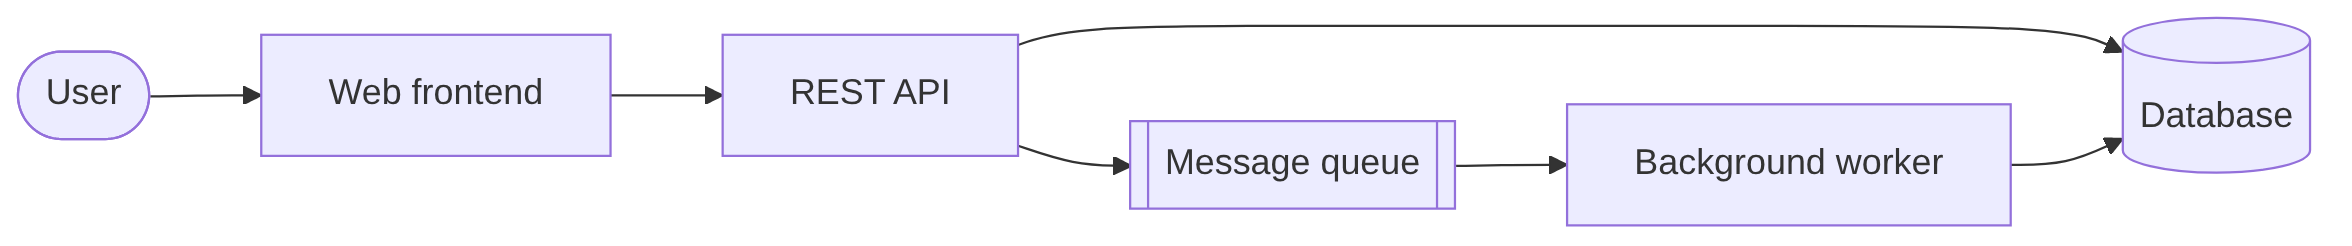
\includegraphics[width=0.85\textwidth]{assets/diagrams/architecture.png}
    \caption{High-level system architecture (Mermaid source:
    \texttt{assets/diagrams/architecture.mmd}).}
    \label{fig:architecture}
\end{figure}

\section{Login flow}
\label{sec:design-login}

Figure~\ref{fig:sequence-login} traces the messages exchanged during a
successful login. The API verifies the supplied password against the
hash retrieved from the database before issuing a session token.

\begin{figure}[H]
    \centering
    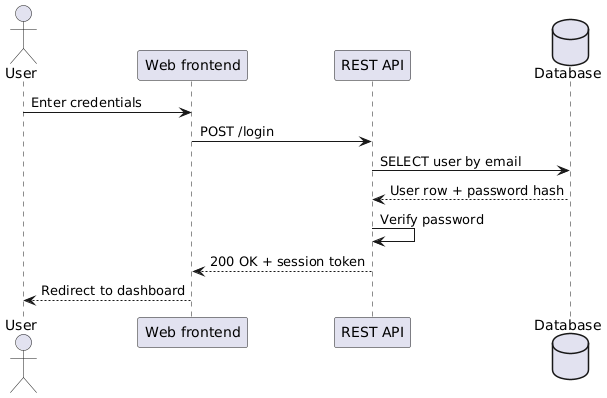
\includegraphics[width=0.85\textwidth]{assets/diagrams/sequence-login.png}
    \caption{Login sequence (PlantUML source:
    \texttt{assets/diagrams/sequence-login.puml}).}
    \label{fig:sequence-login}
\end{figure}
